\usepackage[english]{babel} %language selection
\selectlanguage{english}
\usepackage{makeidx}
\usepackage{graphicx}
\usepackage{rotating}
\usepackage{amsmath,amssymb,amsthm,amscd,mathtools}
\usepackage{color}
\usepackage{enumitem}
\usepackage{ulem}
\usepackage[font=small,labelfont=bf]{caption}
\usepackage{subcaption}
\usepackage{tikz}
\tikzset{dot/.style={draw,shape=circle,fill=black,scale=.2}}
\usepackage{geometry}
\usepackage[pdftex]{hyperref}  %It has been claimed that hyperref should be loaded last...
\hypersetup{ %
  colorlinks=true, %
  linkcolor=red,%  %% links within the doc e.g. ToC entries
  urlcolor=blue,%  %% links to the interwebs
  plainpages=false, %
  pdftitle={Tech Fluency Labs for Math and Science Students, Version 0.1}, %
  pdfauthor={Len Brin, Joe Fields, Younhee Lee and Ray Mugno}, %
  pdfsubject={Computational tools for mathematics} %
}
\pdfcompresslevel=9

\makeatletter
\newcommand{\newreptheorem}[2]{\newtheorem*{rep@#1}{\rep@title}\newenvironment{rep#1}[1]{\def\rep@title{#2 \ref{##1}}\begin{rep@#1}}{\end{rep@#1}}}
\makeatother


\newcommand{\cents}{\textcent\kern 5pt}

\newcommand{\sageprompt}{ {\tt sage$>$} }
\newcommand{\tab}{\rule{20pt}{0pt}}
\newcommand{\blnk}{\rule{1.5pt}{0pt}\rule{.4pt}{1.2pt}\rule{9pt}{.4pt}\rule{.4pt}{1.2pt}\rule{1.5pt}{0pt}}
\newcommand{\suchthat}{\; \rule[-3pt]{.25pt}{13pt} \;}
\newcommand{\divides}{\!\mid\!}
\newcommand{\tdiv}{\; \mbox{div} \;}
\newcommand{\restrict}[2]{#1 \,\rule[-4pt]{.125pt}{14pt}_{\,#2}}
\newcommand{\lcm}[2]{\mbox{lcm} (#1, #2)}
\renewcommand{\gcd}[2]{\mbox{gcd} (#1, #2)}
\newcommand{\Naturals}{{\mathbb N}}
\newcommand{\Integers}{{\mathbb Z}}
\newcommand{\Znoneg}{{\mathbb Z}^{\mbox{\tiny noneg}}}
\newcommand{\Enoneg}{{\mathbb E}^{\mbox{\tiny noneg}}}
\newcommand{\Qnoneg}{{\mathbb Q}^{\mbox{\tiny noneg}}}
\newcommand{\Rnoneg}{{\mathbb R}^{\mbox{\tiny noneg}}}
\newcommand{\Rationals}{{\mathbb Q}}
\newcommand{\Reals}{{\mathbb R}}
\newcommand{\Complexes}{{\mathbb C}}
%\newcommand{\F2}{{\mathbb F}_{2}}
\newcommand{\relQ}{\mbox{\textsf Q}}
\newcommand{\relR}{\mbox{\textsf R}}
\newcommand{\nrelR}{\mbox{\raisebox{1pt}{$\not$}\rule{1pt}{0pt}{\textsf R}}}
\newcommand{\relS}{\mbox{\textsf S}}
\newcommand{\relA}{\mbox{\textsf A}}
\newcommand{\Dom}[1]{\mbox{Dom}(#1)}
\newcommand{\Cod}[1]{\mbox{Cod}(#1)}
\newcommand{\Rng}[1]{\mbox{Rng}(#1)}

\DeclareMathOperator\caret{\raisebox{1ex}{$\scriptstyle\wedge$}}

\newtheorem*{defi}{Definition}
\newtheorem*{exer}{Exercise}
\newtheorem{thm}{Theorem}[section]
\newtheorem*{thm*}{Theorem}
\newtheorem{lem}[thm]{Lemma}
\newtheorem{cor}{Corollary}
\newtheorem{conj}{Conjecture}

\renewenvironment{proof}%
{\begin{quote} \emph{Proof:} }%
{\rule{0pt}{0pt} \newline \rule{0pt}{15pt} \hfill Q.E.D. \end{quote}}

\newenvironment{worksheet}[3]{%
\begin{tabular*}{6in}{l @{\extracolsep{\fill}} r} \hline %
\begin{tabular}[c]{l} %
 {\huge Lab: #1} \\%    %% #1 is a sequence number (should be done automagically, but...  reasons)
{\rule{0pt}{22pt}\LARGE #2} \\%        %% #2 is the title of the activity
\end{tabular} &  \begin{tabular}[c]{r} %
\rule{0pt}{1.05in}\includegraphics[height=1in]{#3} \\%  %% #3 is a thumbnail image for the activity
\end{tabular}  \\ \hline%
\end{tabular*}%
\par \rule{0pt}{6pt} \par \noindent }{ \vfill \centering 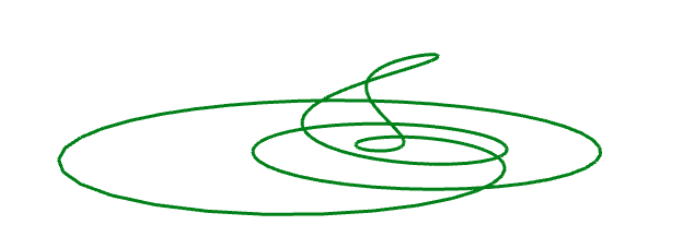
\includegraphics[height=1in, width=5in]{lab_end.png} \clearpage}

\newenvironment{codeblock}{ \par \rule{0pt}{12pt} \par \hfill \begin{minipage}{0.9\textwidth} }{ \end{minipage} \par \rule{0pt}{12pt} \par }

\renewcommand{\baselinestretch}{1.2}
\renewcommand{\arraystretch}{.83}

\graphicspath{{../figures}{figures}}

